\documentclass[12pt]{article}

\usepackage{sbc-template}
\usepackage{graphicx,url}
\usepackage[utf8]{inputenc}

\usepackage{verbatim}
\usepackage{xspace}
\newcommand{\FC}       {Freechains\xspace}
\newcommand{\AMT}      {\emph{AM-Tools}\xspace}
\newcommand{\reps}     {\emph{reps}\xspace}
\newcommand{\onerep}   {\emph{1~rep}\xspace}
\newcommand{\nreps}[1] {\emph{#1~reps\xspace}}
\newcommand{\code}[1]  {\texttt{\footnotesize{#1}}}
\newcommand{\Xon} {$1{\rightarrow}N$\xspace}
\newcommand{\Xno} {$1{\leftarrow}N$\xspace}
\newcommand{\Xnn} {$N{\leftrightarrow}N$\xspace}
\newcommand{\Xoo} {$1{\leftrightarrow}1$\xspace}
\newcommand{\Xo}  {$1{\hookleftarrow}$\xspace}

\newcommand{\amrw}       {\texttt{AM-rw}\xspace}
\newcommand{\amdiff}     {\texttt{AM-diff}\xspace}
\newcommand{\ampatch}    {\texttt{AM-patch}\xspace}
\newcommand{\amcheckout} {\texttt{AM-checkout}\xspace}
\newcommand{\amcommit}   {\texttt{AM-commit}\xspace}

\renewcommand{\theenumi}{\alph{enumi}}

\hyphenation{off-line}

\sloppy

\title{
    \AMT - Operating Permissionless JSON Datasets
}

\author{Anonymous}
\address{Anonymous}

\begin{document}

\begin{comment}
- 8 paginas
- Descrição e motivação do problema resolvido pela ferramenta;
- Arquitetura da solução e descrição das principais funcionalidades;
- Descrição da demonstração planejada para o Salão de Ferramentas, informando equipamentos necessários para tal;
- URL onde a ferramenta está disponível (obrigatório na modalidade Código Aberto);
- URL dos manuais e documentação da ferramenta, incluindo informações e requisitos para instalação (obrigatório na modalidade Código Aberto);
- URL com um vídeo explicando a instalação e as funcionalidades da ferramenta (obrigatório na modalidade Código Fechado e opcional na modalidade Código Aberto).
\end{comment}

\maketitle

\begin{abstract}
Networked collaborative applications, such as Google Docs and Github, allow
users to work together concurrently.
These applications rely on distributed datasets, such as documents and code,
which users expect to see and share in a consistent way.
However, most practical collaborative systems rely on centralized authorities
to ensure data consistency and correctness.
%
In this work, we propose \AMT, a set of tools to manipulate JSON datasets in a
permissionless P2P environment in which users participate in a consensus
mechanism to ensure consistency and correctness.
%
\AMT reconcile Automerge, a JSON-based CRDT, with Freechains, a blockchain with
a reputation mechanism to moderate datasets.
%
\AMT resembles a distributed version control system (DVCS), but with a
consensus mechanism to merge conflicting editions while preserving data
correctness.
\end{abstract}

\section{Introduction}
\label{sec.introduction}

Networked collaborative applications allow remote users to share projects while
working together concurrently \cite{wu2010partial}.
Examples of collaborative applications include Google Docs, Github and
Wikipedia.
%
These applications rely on distributed datasets, such as documents and code,
which are read, written, stored, and synchronized through the network.
In this work, we use generic JSON files to represent datasets, given that they
are human readable and widely adopted as an interchange format.
Users expect to see and share these JSON datasets in a consistent way, even if
their machines synchronize sporadically and at different times.

Currently, most practical collaborative systems rely on centralized authorities
to ensure data consistency and correctness.
However, centralized authorities concentrate too much power, since they control
data ownership and service availability~\cite{pincheira2022decentralized}.
As an emerging alternative, P2P systems~\cite{androutsellis2004survey} aim to
decentralize control, such that applications grow organically with new
users~\cite{rodrigues2010peer}, who contribute with storage, availability, and
also, in our context, with moderation of the datasets.

However, P2P systems strive to ensure data consistency and correctness,
particularly in the presence of malicious users or
Sybils~\cite{douceur2002sybil}.
For instance, malicious users may abuse the system by vandalizing datasets with
SPAM or hate speech.
By consistency, we mean that all replicas reach the same state, while by
correctness, we mean that such consistent state must also be immune to
vandalism (integrity) and preserve the users intent
(accuracy)~\cite{litt2022peritext}.
Integrity and accuracy inevitably depend on the subjective judgement of users,
which we refer as \emph{subjective correctness}.

As a solution to preserve consistency and accuracy is to rely on conflict-free
replicated data types (CRDTs)~\cite{shapiro2011conflict}.
As an example, Automerge~\cite{kleppmann2018automerge} provides JSON data
structures as CRDTs, such that they can be read and written concurrently
without conflicts.
Nevertheless, CRDTs are still subject to corner cases, such as simultaneous
editions of the very same part of datasets.
In addition, CRDTs are not themselves immune to malicious users and Sybils,
which might vandalize datasets with no restrictions, thus affecting their
integrity.
%In such cases, a consensus mechanism might still be necessary to preserve data
%integrity.

\begin{comment}
As a partial solution to preserve integrity, permissioned P2P systems opt for a
centralized authority to grant membership to new users.
Examples of permissioned P2P networks include Ripple~\cite{schwartz2014ripple}
and Hyperledger Fabric~\cite{androulaki2018hyperledger}.
%
Nevertheless, our goal is for a permissionless environment that requires no
centralized membership authority, preserving the organic growth of traditional
P2P systems.
\end{comment}

In a permissionless context, a major challenge is to support concurrent data
edition and moderation, such that users share consistent and correct datasets
even in the presence of Sybils.
%
Bitcoin~\cite{nakamoto2008bitcoin} is a Sybil-resistant permissionless protocol
because it is expensive to write to its unique timeline (either via
proof-of-work or transaction fees).
However, Bitcoin and cryptocurrencies in general provide no subjective means to
moderate conflicts in collaborative datasets, but instead rely on tokens to
arbitrate conflicts.
%
As an alternative targeting collaborative applications,
Freechains~\cite{sant2020freechains} resists Sybils through a reputation
mechanism that moderates content through likes and dislikes and, at the same
time, delivers network consensus.
However, unlike CRDTs and Automerge, Freechains does not support operations on
structured datasets, such as the JSON format.

In this work, we propose \AMT, a set of tools that reconciles Automerge and
Freechains, extending JSON CRDTs with a consensus mechanism that can handle
correctness corner cases and also moderate malicious editions:
Automerge editions are ordered by the Freechains consensus mechanism providing
a priority to resolve conflicts, thus preserving accuracy.
In addition, further moderation can revert priorities or even remove abusive or
malicious editions, thus preserving integrity.
%
A dataset is structured as Automerge JSON file stored on Freechains.
Each file is a separate blockchain that stores a list of modifications to the
JSON.
The list is traversed from the beginning in consensus order to recreate the
file as a complete JSON.
%
In this sense \AMT resembles a distributed version control system (DVCS), but
with a consensus mechanism to merge conflicting editions while
preserving data correctness.

\AMT is composed of 3 utilities:
    \amrw,
    \amdiff \& \ampatch, and
    \amcheckout \& \amcommit.
%
\amrw allows to read and write portions of a JSON file.
\amdiff \& \ampatch obtain and apply differences between JSON files.
\amcheckout \& \amcommit read and write a JSON file to its corresponding
blockchain.

The rest of this paper is organized as follows.
Sections~\ref{sec.automerge}~and~\ref{sec.freechains} describe the basic
functionality of Automerge and Freechains as separate tools, highlighting how
they form the basis of \AMT.
Section~\ref{sec.amtools} describes \AMT and how it combines Automerge and
Freechains.

\section{Automerge}
\label{sec.automerge}

Automerge~\cite{kleppmann2018automerge} is an open-source library that provides
CRDT-based JSON datasets to build collaborative applications.
%
Automerge is designed for \emph{local-first software}~\cite{p2p.local} which,
unlike cloud-based software, stores and operates the datasets locally, such
that applications can work normally while offline.
%
Therefore, users can make concurrent changes to a shared JSON without
centralized coordination:
When users synchronize, Automerge ensures that changes are merged automatically
in a principled manner.
%
More specifically, Automerge is an operation-based CRDT
(CmRDT~\cite{p2p.crdts}) that models JSON datasets as append-only logs of
concurrent commutative modifications, such as the insertion or removal of list
elements~\cite{kleppmann2017conflict}.
%
When users synchronize, these logs are merged to reach the exactly same state
according to the eventual consistency model~\cite{p2p.sec}.

The basic JavaScript API of Automerge is as follows:

\begin{itemize}
\item \code{obj = AM.init()} \\
    Initializes a JSON as an empty object \code{obj=\{\}}.
\item \code{obj2 = AM.change(obj1, f)} \\
    Modifies object \code{obj1} through function \code{f}, resulting in
    object \code{obj2}.
\item \code{chgs = AM.getChanges(obj1, obj2)} \\
    Compares objects \code{obj1} and \code{obj2}, resulting in changes
    \code{chgs}.
\item \code{obj2 = AM.applyChanges(obj1, chgs)} \\
    Applies changes \code{chgs} to object \code{obj1}, resulting in object
    \code{obj2}.
\item \code{errs = AM.getConflicts(obj, fld)} \\
    Checks merge conflicts in field \code{fld} of object \code{obj}, resulting
    in a set \code{errs}.
\item \code{bin = AM.save(obj)} \\
    Converts object \code{obj} to a byte array \code{bin}.
\item \code{obj = AM.load(bin)} \\
    Converts a byte array \code{bin} to object \code{obj}.
\end{itemize}

Note that the basic API of Automerge is network agnostic and does not provide
a mechanism to synchronize objects, requiring extra libraries for this purpose.
%
This apparent limitation matches our intention to adopt Freechains as a
transport and storage layer with global consensus.

The API usage is straightforward:
    initialize a dataset with \code{AM.init},
    make local changes with \code{AM.change} and \code{AM.getChanges},
    synchronize with other users (extra),
    apply remote changes with \code{AM.applyChanges},
    check conflicts with \code{AM.getConflicts},
    persist locally with \code{AM.save} and \code{AM.load}.
Except for function \code{AM.change}, the other functions are straightforward.
%
Because Automerge is a CmRDT and must keep track of all operations, JSON
objects cannot be manipulated directly in JavaScript.
Instead, \code{AM.change} receives a function argument to manipulate
the given object with tracking enabled.

Regarding \AMT,
    \code{AM.init} and \code{AM.change} are the basis of \amrw;
    \code{AM.getChanges}, \code{AM.applyChanges}, and \code{AM.getConflicts}
    are the basis of \amdiff \& \ampatch; and
    \code{AM.save} and \code{AM.load} are used for persistence in
    \amcheckout \& \amcommit.

The next example simulates two peers \code{A} and \code{B} manipulating a
JSON concurrently to reach the final state \code{\{list:~['A','B']\}}:

\noindent
{\footnotesize
\begin{minipage}[t]{0.6\textwidth}
\begin{verbatim}
// PEER A
A1 = AM.init()
A2 = AM.change(A1, json => {
    json.list = []
})

X0 = AM.getChanges(A1,A2)   --sync-X0-->

A3 = AM.change(A2, json => {
    json.list.push('A')
})

XA = AM.getChanges(A2,A3)   <--XB--XA-->
A4 = AM.applyChanges(A3, XB)
\end{verbatim}
\end{minipage}
\begin{minipage}[t]{0.4\textwidth}
\begin{verbatim}
// PEER B
B1 = AM.init()




B2 = AM.applyChanges(B1, X0)

B3 = AM.change(B2, json => {
    json.list.push('B')
})

XB = AM.getChanges(A2,A3)
B4 = AM.applyChanges(B3, XA)
\end{verbatim}
\end{minipage}
}

Peers \code{A} and \code{B} initialize a new JSON independently (\code{A1} and
\code{B1}).
Then, peer \code{A} adds an empty list (\code{A2}), computes the difference
(\code{X0}), and synchronizes it with peer \code{B} (\code{B2}).
Then, both peers push values to the list concurrently (\code{A3} and
\code{B3}), and synchronize the differences (\code{XA} and \code{XB}), which
are applied in the other sides (\code{A4} and \code{B4}).
Automerge ensures that the final states \code{A4} and \code{B4} are exactly the
same, with the list containing both values \code{'A'} and \code{'B'}.
However, since the editions are concurrent, the final list may become either
\code{['A','B']} or \code{['B','A']}, depending on arbitrary criteria such as
peer identity or timestamp.
Nevertheless, regardless of the order, the users intent to push two values into
the list is preserved.

Now, suppose that instead of calls to \code{json.list.push}, the peers set the
lists directly as \code{json.list=['A']} and \code{json.list=['B']}.
In this case, the concurrent assignments are incompatible, and an
irreconcilable conflict occurs.
Nevertheless, Automerge arbitrarily chooses one of the assignments, but still
detects and indicates the conflict through \code{AM.getConflicts}.
Note that for such corner cases, Automerge does not preserve accuracy, since
the intent of one of the users is not satisfied.

In addition, since Automerge does not rule over peer synchronization, it cannot
enforce data integrity either.
For instance, a priori, nothing stops malicious users from vandalizing the
datasets with SPAM or erroneous information.
%
Therefore, even though Automerge provides a solid foundation for
eventually-consistency JSON datasets, it cannot ensure integrity and accuracy
in all cases, specially in a permissionless environment.

\section{Freechains}
\label{sec.freechains}

Freechains~\cite{fcs.sbseg20} is a content dissemination P2P protocol in which
all users observe the same total order of messages through a consensus
mechanism.
%
Users post messages to a topic or chain and other users subscribed to the same
chain eventually receive the messages.
%
Each chain behaves as an independent blockchain with an innovative reputation
mechanism that moderates content through likes and dislikes and, at the same
time, delivers consensus.
%
Figure~\ref{fig.general} summarizes the general reputation rules, in which
users can spend tokens named \emph{reps} to post and rate content in the
chains:
    a post initially penalizes authors until it consolidates and counts positively;
    a like is a positive feedback that helps subscribers to distinguish content amid excess;
    a dislike is a negative feedback that revokes content when crossing a threshold.

\begin{figure}
    \centering
    \begin{minipage}{0.60\textwidth}
        \centering
        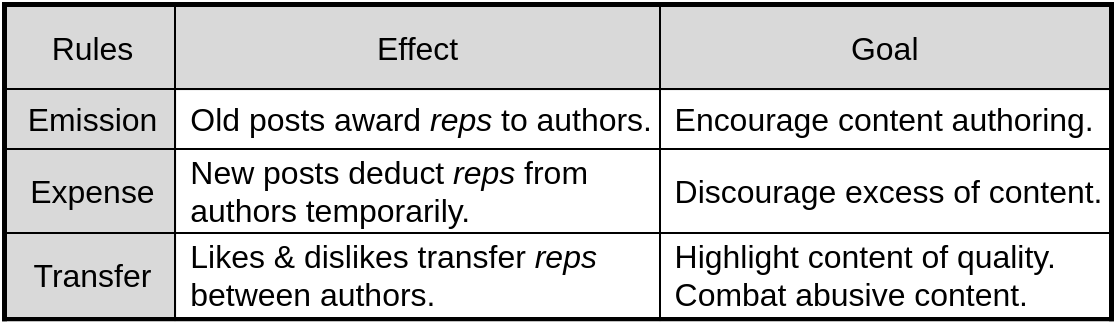
\includegraphics[width=\textwidth]{general.png}
        \caption{General reputation rules in public chains.}
        \label{fig.general}
    \end{minipage}\hfill
    \begin{minipage}{0.40\textwidth}
        \centering
        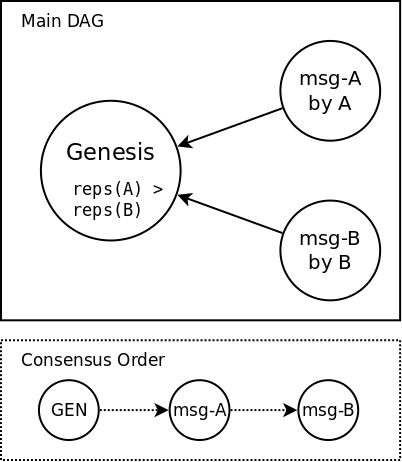
\includegraphics[width=0.9\textwidth]{dag.png}
        \caption{A chain DAG with corresponding consensus order.}
        \label{fig.dag}
    \end{minipage}
\end{figure}

The reputation mechanism of Freechains works towards our goal of subjective
correctness in \AMT as follows:
    dislikes can revoke abusive and malicious posts, thus preserving integrity;
    likes can favor posts with more quality, thus preserving accuracy.

The basic command-line API of Freechains is as follows:

\begin{itemize}
\item \code{fc keys ...} \\
    Creates cryptographic keys as user identities.
\item \code{fc chains join ...} \\
    Joins a chain to post and read content.
\item \code{fc chain post ...} \\
    Posts a message to a chain.
\item \code{fc chain get ...} \\
    Reads a post from a chain.
\item \code{fc chain like ...} \\
    Likes (or dislikes) a post in the chain.
\item \code{fc chain consensus ...} \\
    Shows all posts from a chain in consensus order.
\item \code{fc peer sync ...} \\
    Synchronizes a chain with a remote peer.
\end{itemize}

Except for \code{fc~peer~sync}, none of the commands connect to the network,
but only modify the local replica.
%
Users need to call \code{fc~keys} only once to create a public-private key pair
as an identity to operate in the chains.
%
For each chain of interest, users need to call \code{fc~chains~join} with the
same arguments such that they are compatible when synchronizing.
%
Once a chain is created, users can call \code{fc~chain~get} and
\code{fc~chain~post} to read and write messages.
%
A chain can be traversed in order through \code{fc~chain~consensus}, which
enumerates all post ids, which can be read through \code{fc~chain~get}.
%
Finally, \code{fc~peer~sync} exchanges missing posts between replicas.

Regarding \AMT, we use \code{fc~chain~post/get} to persist Automerge operations
serialized through \code{AM.save} and \code{AM.load}.
We also rely on \code{fc~peer~sync} as a synchronization layer to Automerge,
but with integrity and accuracy via \code{fc~chain~consensus}.

Like Automerge, Freechains is also designed for
\emph{local-first software}~\cite{p2p.local}, given that most commands only
modify the local replica.
For this reason, concurrent posts are not only encouraged, but are also
inevitable.
The next example simulates two users \code{A} and \code{B} posting concurrently
to chain \code{\#p2p}:

\noindent
{\footnotesize
\begin{minipage}[t]{0.5\textwidth}
\begin{verbatim}
// USER A
$ fc keys pubpvt 'passwd-A'
<pub-A> <pvt-A>
$ fc chains join '#p2p' \
    <pub-A> <pub-A> <pub-B>
$ fc chain '#p2p' post inline \
    "msg-A" --sign=<pvt-A>
$ fc peer <ip-B> sync '#p2p'
$ fc chain '#p2p' consensus
msg-A --> msg-B
\end{verbatim}
\end{minipage}
\begin{minipage}[t]{0.5\textwidth}
\begin{verbatim}
// USER B
$ fc keys pubpvt 'passwd-B'
<pub-B> <pvt-B>
$ fc chains join '#p2p' \
    <pub-A> <pub-A> <pub-B>
$ fc chain '#p2p' post inline \
    "msg-B" --sign=<pvt-B>
$ fc peer <ip-A> sync '#p2p'
$ fc chain '#p2p' consensus
msg-A --> msg-B
\end{verbatim}
\end{minipage}
}

Users \code{A} and \code{B} first generate their identities and join the
public chain \code{\#p2p} with the same arguments.
The keys after \code{join~'\#p2p'} represent the pioneers, which share an
initial reputation to moderate the chain.
In the example, we determine that user \code{A} has twice of \code{B}'s
reputation in order to illustrate the consensus mechanism of Freechains.
Then, the users call \code{chain~post} concurrently with distinct messages and
signatures, which creates a fork in the chain.
%
After the users synchronize with \code{peer~sync}, the posts are exchanged and
the chain reaches the state of Figure~\ref{fig.dag}.
The chain fork represented in the DAG suggests that only a partial order of
posts is possible.
Nevertheless, the call to \code{chain~consensus} always returns the same order
of posts \code{msg-A~-->~msg-B} in both sides.

The consensus algorithm of Freechains provides a total order of posts, even in
the presence of forks.
Freechains employs a topological sorting algorithm to favor reputation when
deciding between branches in a chain DAG.
The algorithm works as follows~\cite{fcs.sbseg20}:
\begin{itemize}
\item
    The common prefix is evaluated to extract the reputation of all users with
    posts.
    In Figure~\ref{fig.dag}, the common prefix only contains the genesis
    block, in which user \code{A} has more reputation than user \code{B}.
\item
    Each branch in the fork is evaluated to extract the set of users with
    posts.
    In Figure~\ref{fig.dag}, the branch at the top contains user \code{A} and
    the branch at the bottom contains user \code{B}.
\item
    The branches are ordered based on the sum of reputation of their users, but
    considering the common prefix.
    In Figure~\ref{fig.dag}, user \code{A} had more reputation in the common
    prefix, therefore, the branch at the top is ordered first.
\end{itemize}

Even though Freechains provide means to preserve integrity and accuracy, it
does not support structured datasets with attached semantics, since it
represents content as a simple linked list of binary blobs stored in chains.

\section{AM-Tools}
\label{sec.amtools}

\AMT reconciles Automerge and Freechains to provide a solid foundation to
manipulate JSON datasets in permissionless networks, while preserving
consistency, integrity, and accuracy.
%
On the one hand, Automerge supports decentralized high-level structured JSON
datasets with fine-grained merging policies, but which are still subject to
integrity abuse and corner-case inaccuracies.
%
On the other hand, Freechains can resist malicious peers and order conflicting
corner cases, but does not support structured datasets with merging policies.

As described in the Introduction, \AMT is composed of 3 utilities:
    \amrw,
    \amdiff \& \ampatch, and
    \amcheckout \& \amcommit.
%
\amrw allows to read and write portions of a JSON file.
\amdiff \& \ampatch obtain and apply differences between JSON files.
\amcheckout \& \amcommit read and write a JSON file to its corresponding
blockchain.

\subsection{\amrw: JSON Command-Line Editor}

\amrw%
    %\footnote{\amrw: \url{https://github.com/fabiobosisio/amrw}}
    \footnote{\amrw: \url{https://github.com/<hidden-anonymous>}}
is a facade to hide the complexity of \code{AM.change}, and also provide a
uniform syntax to manipulate JSON files.
Recall from Section~\ref{sec.automerge} that, because CmRDTs need to keep
track of all operations, JSON files cannot be edited directly.

The basic command-line API of \amrw is as follows:

\begin{itemize}
\item \code{AM-rw <file> init} \\
    Initializes a file as an empty JSON object (based on \code{AM.init}).
\item \code{AM-rw <file> <path>... (read | write <op>)} \\
    Reads a value from or writes to a JSON file (based on \code{AM.change}).
    A \code{<path>...} is a sequence of field or index accesses to navigate the
    JSON.
    A \code{write <op>} can insert, set, or remove a field or index from the
    JSON.
\end{itemize}

The next example initializes and writes to a JSON to reach the final state
{list: ['A','B']}:

\begin{verbatim}
$ AM-rw "test.am" init
$ AM-rw "test.am" write object ins "list" array
$ AM-rw "test.am" field "list" write array ins 0 string "A"
$ AM-rw "test.am" field "list" write array ins 1 string "B"
$ AM-rw "test.am" read
{ list: [ 'A', 'B' ] }
\end{verbatim}

In the first write, we use an empty path, which navigates to the root object,
in which we add a field \code{list} as an empty array.
The writes in sequence navigate to the array in field \code{list}, and insert
strings \code{A} and \code{B}.

Even though \amrw is more verbose in comparison to Automerge's
\code{AM.change}, it provides a uniform syntax to manipulate JSON files.
In addition, as a command-line tool, it can be used from outside JavaScript
even by non programmers.

\subsection{\amdiff \& \ampatch}

\amdiff \& \ampatch%
    %\footnote{\ampatch: \url{https://github.com/fabiobosisio/ampatch}}
    \footnote{\amdiff \& \ampatch: \url{https://github.com/<hidden-anonymous>}}
are counterparts to textual \emph{diff \& patch} UNIX tools, but for
Automerge's JSON internal format.

The basic command-line API of \amdiff \& \ampatch is as follows:

\begin{itemize}
\item \code{AM-diff <old> <new>} \\
    Calculates the differences between the given files.
\item \code{AM-patch <cur> <patch>} \\
    Applies the patch to the given file.
\end{itemize}

The next example illustrates how to extract the differences between an old and
a new file, and then recreate the new file by applying the obtained difference
into the old file:

\begin{verbatim}
$ AM-diff  "old.am" "new.am" > "old-new.diff"
$ AM-patch "old.am" "old-new.diff" > "rec.am"
\end{verbatim}

At the end, \code{new.am} and \code{rec.am} must be equal files.

Just like standard version control systems, the idea is that storing
\emph{diffs} to recreate the full history of a given file history is more
efficient than storing all individual versions of that file.

With \AMT, we support a permissionless environment built on top of Freechains
to store these file \emph{diffs}, which users can rate and possibly revoke,
affecting the consensus order to recreate the file history.

\subsection{\amcheckout \& \amcommit}

The final missing piece of \AMT is to synchronize JSON files between replicas
and then update the local version based on the global consensus.

\amcheckout \& \amcommit%
    %\footnote{\amcheckout \& \amcommit: \url{https://github.com/fabiobosisio/ampatch}}
    \footnote{\amcheckout \& \amcommit: \url{https://github.com/<hidden-anonymous>}}

\begin{verbatim}
AM-freechains (checkout|commit) <chain> <file> --sign=<pvt>
\end{verbatim}


facade is an object that serves as a front-facing interface masking more complex underlying or structural code. A facade can:

\bibliographystyle{abbrv}
\bibliography{amtools}

\end{document}
